% Archivo: portada.tex
\thispagestyle{empty} % Deshabilitamos encabezado y pie para la portada
\fancyhf{} % Limpiamos los encabezados y pies de página
\renewcommand{\headrulewidth}{0pt} % Sin línea en el encabezado
\renewcommand{\footrulewidth}{0pt} % Sin línea en el pie de página

\begin{table}[H]
\begin{minipage}[t][0.8\paperheight][s]{0.08\columnwidth}%
\noindent \vspace{0cm}
\begin{flushright}
    
\includegraphics[scale=0.8]{CAPITULOS/PORTADA/ipn.png} \\[5mm]
    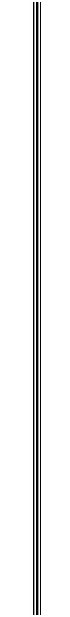
\includegraphics[scale=1.5]{CAPITULOS/PORTADA/barra2} \\[5mm]
    
\includegraphics[scale=0.3]{CAPITULOS/PORTADA/upiita}
\end{flushright}%
\end{minipage}\hfill{}%
\begin{minipage}[t][0.8\paperheight][s]{0.86\columnwidth}%
\begin{center}
    \textbf{\huge Instituto Politécnico Nacional} \\[1cm]
    \textbf{\Large Unidad Profesional Interdisciplinaria en Ingeniería y Tecnologías Avanzadas} \\[1cm]
    \textbf{\large Proyecto Terminal 1} \\[1cm]
    {\large Sistema de reconocimiento de señas de detección de palabras para el lenguaje de señas LSM} \\[1cm]
    \emph{Que para obtener el título de} \\[1cm]
    \textbf{\large ``Ingeniero en Telemática''} \\[1cm]
    \emph{Presenta:} \\[1cm]
    {\large Jose Daniel Alvarez Ramos} \\[1cm]
    \emph{Asesor(es):} \\[1cm]
    {\large Dr. en C. Bella C. Martínez Seis} \\[1cm]
\end{center}
\end{minipage}

% Añadimos el texto alineado a la derecha a la altura de la imagen "upiita"
\vspace{-2cm} % Ajustamos este valor para alinearlo con la imagen
\begin{flushright}
    \textit{México,CDMX, a 10 de octubre de 2024.}
\end{flushright}
\end{table}

\newpage % Nueva página después de la portada
